\documentclass{standalone}
\usepackage{tikz}
\usetikzlibrary{patterns, positioning}
\usepackage[sfdefault]{ClearSans} %% option 'sfdefault' activates Clear Sans as the default text font
\usepackage[T1]{fontenc}

\begin{document}
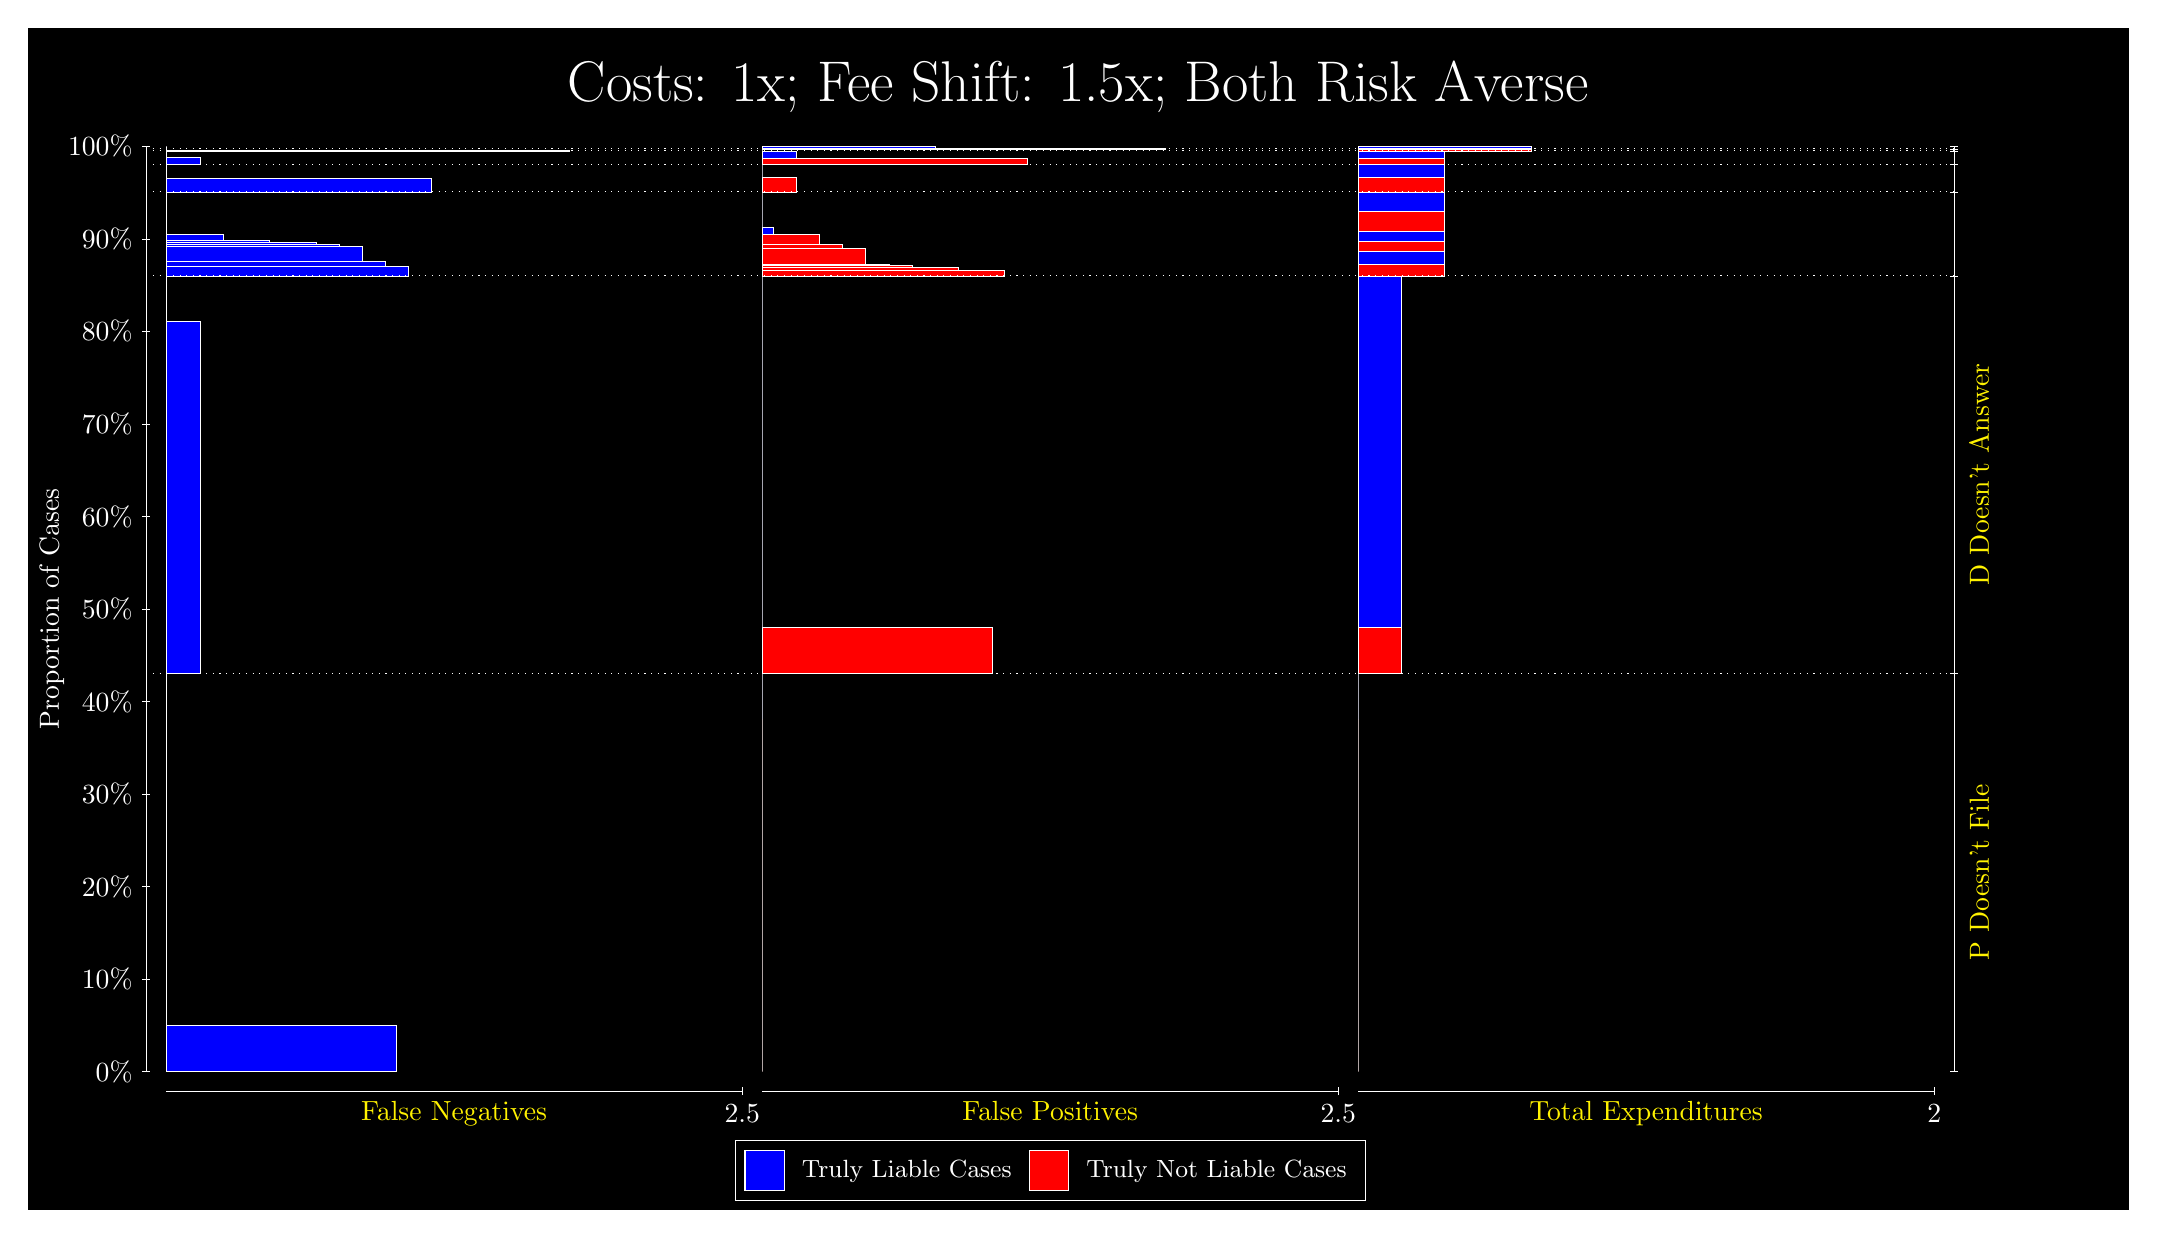
\begin{tikzpicture}
\draw[fill=black] (0,0) rectangle (26.667,15);
\draw[text=white] (0,13.5) rectangle (26.667,15) node[midway] {\huge Costs: 1x; Fee Shift: 1.5x; Both Risk Averse};
\draw[white, very thin] (1.5,1.75) -- (1.5,13.5);
\node[rotate=90, text=white, anchor=center] at (0.3, 7.625) {Proportion of Cases};
\draw[white, very thin] (1.45,1.75) -- (1.55,1.75);
\node[text=white, anchor=east] at (1.45, 1.75) {0\%};
\draw[white, very thin] (1.45,2.925) -- (1.55,2.925);
\node[text=white, anchor=east] at (1.45, 2.925) {10\%};
\draw[white, very thin] (1.45,4.1) -- (1.55,4.1);
\node[text=white, anchor=east] at (1.45, 4.1) {20\%};
\draw[white, very thin] (1.45,5.275) -- (1.55,5.275);
\node[text=white, anchor=east] at (1.45, 5.275) {30\%};
\draw[white, very thin] (1.45,6.45) -- (1.55,6.45);
\node[text=white, anchor=east] at (1.45, 6.45) {40\%};
\draw[white, very thin] (1.45,7.625) -- (1.55,7.625);
\node[text=white, anchor=east] at (1.45, 7.625) {50\%};
\draw[white, very thin] (1.45,8.8) -- (1.55,8.8);
\node[text=white, anchor=east] at (1.45, 8.8) {60\%};
\draw[white, very thin] (1.45,9.975) -- (1.55,9.975);
\node[text=white, anchor=east] at (1.45, 9.975) {70\%};
\draw[white, very thin] (1.45,11.15) -- (1.55,11.15);
\node[text=white, anchor=east] at (1.45, 11.15) {80\%};
\draw[white, very thin] (1.45,12.325) -- (1.55,12.325);
\node[text=white, anchor=east] at (1.45, 12.325) {90\%};
\draw[white, very thin] (1.45,13.5) -- (1.55,13.5);
\node[text=white, anchor=east] at (1.45, 13.5) {100\%};

\draw[white, very thin] (24.457,1.75) -- (24.457,13.5);
\draw[white, very thin] (24.407,1.75) -- (24.507,1.75);
\node[anchor=west] at (24.407, 1.75) {};
\draw[white, very thin] (24.407,6.8105) -- (24.507,6.8105);
\node[anchor=west] at (24.407, 6.8105) {};
\draw[white, very thin] (24.407,11.854) -- (24.507,11.854);
\node[anchor=west] at (24.407, 11.854) {};
\draw[white, very thin] (24.407,12.922) -- (24.507,12.922);
\node[anchor=west] at (24.407, 12.922) {};
\draw[white, very thin] (24.407,13.273) -- (24.507,13.273);
\node[anchor=west] at (24.407, 13.273) {};
\draw[white, very thin] (24.407,13.443) -- (24.507,13.443);
\node[anchor=west] at (24.407, 13.443) {};
\draw[white, very thin] (24.407,13.468) -- (24.507,13.468);
\node[anchor=west] at (24.407, 13.468) {};
\draw[white, very thin] (24.407,13.5) -- (24.507,13.5);
\node[anchor=west] at (24.407, 13.5) {};

\draw[white, very thin, fill=blue] (1.75,1.75) rectangle (4.6775,2.3361);
\draw[white, very thin, fill=red] (1.75,2.3361) rectangle (1.75,6.8105);
\draw[white, very thin, fill=blue] (1.75,6.8105) rectangle (2.1891,11.276);
\draw[white, very thin, fill=red] (1.75,11.276) rectangle (1.75,11.854);
\draw[white, very thin, fill=blue] (1.75,11.854) rectangle (4.8239,11.978);
\draw[white, very thin, fill=blue] (1.75,11.978) rectangle (4.5312,12.035);
\draw[white, very thin, fill=blue] (1.75,12.035) rectangle (4.2384,12.229);
\draw[white, very thin, fill=blue] (1.75,12.229) rectangle (3.9457,12.25);
\draw[white, very thin, fill=blue] (1.75,12.25) rectangle (3.6529,12.276);
\draw[white, very thin, fill=blue] (1.75,12.276) rectangle (3.0674,12.307);
\draw[white, very thin, fill=blue] (1.75,12.307) rectangle (2.4819,12.386);
\draw[white, very thin, fill=red] (1.75,12.386) rectangle (1.75,12.922);
\draw[white, very thin, fill=blue] (1.75,12.922) rectangle (5.1167,13.089);
\draw[white, very thin, fill=red] (1.75,13.089) rectangle (1.75,13.273);
\draw[white, very thin, fill=blue] (1.75,13.273) rectangle (2.1891,13.366);
\draw[white, very thin, fill=red] (1.75,13.366) rectangle (1.75,13.443);
\draw[white, very thin, fill=blue] (1.75,13.443) rectangle (6.8732,13.453);
\draw[white, very thin, fill=red] (1.75,13.453) rectangle (1.75,13.468);
\draw[white, very thin, fill=red] (1.75,13.468) rectangle (1.75,13.479);
\draw[white, very thin, fill=blue] (1.75,13.479) rectangle (1.75,13.5);
\draw[white, very thin, fill=red] (9.3189,1.75) rectangle (9.3189,6.2244);
\draw[white, very thin, fill=blue] (9.3189,6.2244) rectangle (9.3189,6.8105);
\draw[white, very thin, fill=red] (9.3189,6.8105) rectangle (12.246,7.388);
\draw[white, very thin, fill=blue] (9.3189,7.388) rectangle (9.3189,11.854);
\draw[white, very thin, fill=red] (9.3189,11.854) rectangle (12.393,11.929);
\draw[white, very thin, fill=red] (9.3189,11.929) rectangle (11.807,11.96);
\draw[white, very thin, fill=red] (9.3189,11.96) rectangle (11.222,11.987);
\draw[white, very thin, fill=red] (9.3189,11.987) rectangle (10.929,12.007);
\draw[white, very thin, fill=red] (9.3189,12.007) rectangle (10.636,12.201);
\draw[white, very thin, fill=red] (9.3189,12.201) rectangle (10.344,12.258);
\draw[white, very thin, fill=red] (9.3189,12.258) rectangle (10.051,12.389);
\draw[white, very thin, fill=blue] (9.3189,12.389) rectangle (9.4652,12.468);
\draw[white, very thin, fill=blue] (9.3189,12.468) rectangle (9.3189,12.922);
\draw[white, very thin, fill=red] (9.3189,12.922) rectangle (9.758,13.106);
\draw[white, very thin, fill=blue] (9.3189,13.106) rectangle (9.3189,13.273);
\draw[white, very thin, fill=red] (9.3189,13.273) rectangle (12.686,13.35);
\draw[white, very thin, fill=blue] (9.3189,13.35) rectangle (9.758,13.443);
\draw[white, very thin, fill=red] (9.3189,13.443) rectangle (9.3189,13.458);
\draw[white, very thin, fill=blue] (9.3189,13.458) rectangle (9.3189,13.468);
\draw[white, very thin, fill=red] (9.3189,13.468) rectangle (14.442,13.479);
\draw[white, very thin, fill=blue] (9.3189,13.479) rectangle (11.515,13.5);
\draw[white, very thin, fill=red] (16.888,1.75) rectangle (16.888,6.2244);
\draw[white, very thin, fill=blue] (16.888,6.2244) rectangle (16.888,6.8105);
\draw[white, very thin, fill=red] (16.888,6.8105) rectangle (17.437,7.388);
\draw[white, very thin, fill=blue] (16.888,7.388) rectangle (17.437,11.854);
\draw[white, very thin, fill=red] (16.888,11.854) rectangle (17.986,12.007);
\draw[white, very thin, fill=blue] (16.888,12.007) rectangle (17.986,12.165);
\draw[white, very thin, fill=red] (16.888,12.165) rectangle (17.986,12.296);
\draw[white, very thin, fill=blue] (16.888,12.296) rectangle (17.986,12.42);
\draw[white, very thin, fill=red] (16.888,12.42) rectangle (17.986,12.671);
\draw[white, very thin, fill=blue] (16.888,12.671) rectangle (17.986,12.922);
\draw[white, very thin, fill=red] (16.888,12.922) rectangle (17.986,13.106);
\draw[white, very thin, fill=blue] (16.888,13.106) rectangle (17.986,13.273);
\draw[white, very thin, fill=red] (16.888,13.273) rectangle (17.986,13.35);
\draw[white, very thin, fill=blue] (16.888,13.35) rectangle (17.986,13.443);
\draw[white, very thin, fill=red] (16.888,13.443) rectangle (19.083,13.458);
\draw[white, very thin, fill=blue] (16.888,13.458) rectangle (19.083,13.468);
\draw[white, very thin, fill=red] (16.888,13.468) rectangle (19.083,13.479);
\draw[white, very thin, fill=blue] (16.888,13.479) rectangle (19.083,13.5);
\draw[white, dotted] (1.5,6.8105) -- (24.457,6.8105);
\draw[white, dotted] (1.5,11.854) -- (24.457,11.854);
\draw[white, dotted] (1.5,12.922) -- (24.457,12.922);
\draw[white, dotted] (1.5,13.273) -- (24.457,13.273);
\draw[white, dotted] (1.5,13.443) -- (24.457,13.443);
\draw[white, dotted] (1.5,13.468) -- (24.457,13.468);
\draw[white, very thin] (1.75,1.5) -- (9.0689,1.5);
\node[text=yellow, anchor=north] at (5.4094, 1.5) {False Negatives};
\draw[white, very thin] (9.0689,1.45) -- (9.0689,1.55);
\node[text=white, anchor=north] at (9.0689, 1.45) {2.5};

\draw[white, very thin] (9.3189,1.5) -- (16.638,1.5);
\node[text=yellow, anchor=north] at (12.978, 1.5) {False Positives};
\draw[white, very thin] (16.638,1.45) -- (16.638,1.55);
\node[text=white, anchor=north] at (16.638, 1.45) {2.5};

\draw[white, very thin] (16.888,1.5) -- (24.207,1.5);
\node[text=yellow, anchor=north] at (20.547, 1.5) {Total Expenditures};
\draw[white, very thin] (24.207,1.45) -- (24.207,1.55);
\node[text=white, anchor=north] at (24.207, 1.45) {2};

\node[text=yellow, centered, rotate=90] at (24.777, 4.2803) {P Doesn't File};
\node[text=yellow, centered, rotate=90] at (24.777, 9.3321) {D Doesn't Answer};






\draw (12.978300999999998,1.5) node[draw=none] (baseCoordinate) {};
\begin{scope}[align=center]
        \matrix[scale=0.5, draw=white, below=0.5cm of baseCoordinate, nodes={draw}, column sep=0.1cm]{
            \node[rectangle, draw, minimum width=0.5cm, minimum height=0.5cm, fill=blue] {}; &
            \node[draw=none, font=\small, text=white] (B) {Truly Liable Cases}; &
            \node[rectangle, draw, minimum width=0.5cm, minimum height=0.5cm, fill=red] {}; &
            \node[draw=none, font=\small, text=white] (B) {Truly Not Liable Cases}; \\
            };
\end{scope}

\end{tikzpicture}
\end{document}